\documentclass{article}
\usepackage[margin=1in]{geometry}
\usepackage{xeCJK}
\usepackage{tikz}
%\usetikzlibrary{graphdrawing}
%\usegdlibrary{arrows}
%\setCJKmainfont{Noto Serif CJK TC}
\title{Graph Theory Homework 1}
\author{Andr\'es Ponce \\
\and
P76107116
}
%\and  Uncomment wwhen using Chinese name
%彭思安}

\begin{document}
\maketitle
\section{(True or False) There exists a simple graph with 6 vertices, whose degrees are $2,3,3,4,4,5$. }
This statement is \textbf{false}.
According to the Degree-Sum Theorem, given a vertex $v$ and its degree $d(v)$, the sum of the degrees is 
twice the number of edges in our graph.
	\begin{equation} 
		\label{eq:DSF}
		\sum_{v\in V(G)} d(v) = 2e(G)
	\end{equation}
When counting the degrees, each edge gets counted exactly twice, since one edge connects one vertex $u$ to another vertex $v$.
The total number of degrees then has to be an even number.
A corollary of this rule is that a graph can have only an even number of vertices with odd degrees, since an even number of odd degrees 
would result in an even degree count.
In the list above, we have three vertices with odd degree, which violates the degree sum rule. 
Such a graph can not exist.

\section{Determine the values of $m,n$ such that a complete bipartite graph $K_{m,n}$ is a complete graph.}
A \textbf{complete graph} is a graph for which there exists an edge between any pair of vertices $u, v, u\neq v$.
In a bipartite graph, the vertices are split into two sets such that their union is $V(G)$.
All the vertices from one partition have an edge to all the vertices in the other partition.

The values $m=1, n=1$ satisfy the constraints.
For the graph $K_{1,1}$, there is an edge connecting every pair of distinct vertices, which satisfies the definition of a complete graph,
and also every node in one partition is connected to all the nodes in the other partition, satisfying the definition of a bipartite graph.

\section{Briefly describe the definition of a simple graph.}
Firstly, a graph $G$ is a of edges $E(G)$ and vertices $V(G)$, where edges connect a pair of endpoints.
A simple graph is a graph that does not have any loops or multiple edges.
Loops are edges with equal endpoints,and multiple edges refer to more than one edge that has the same pair of 
endpoints.

\section{Draw the complement of the following graph}
\begin{equation}
\centering
\begin{tikzpicture}[node distance=5em]
	\node (u) at (0,0) {u};
	\node (y) [below left of=u] {y};
	\node (v) [below right of=u] {v};
	\node (x) [below of=y] {x};
	\node (w) [below of=v] {w};

	\path[-] (u) edge (y);
	\path[-] (u)  edge (v);
	\path[-]  (u) edge  (x);
	\path[-]  (y) edge  (x);
	\path[-]  (v) edge  (w);
	\path[-]  (x) edge  (w);
\end{tikzpicture}
\end{equation}

A graph has a set of vertices $V(G)$ and edges $E(G)$.
The complement $\bar{G}$ of $G$ is defined as the set of edges $u,v\in E(\bar{G})$
if and only if $u,v\notin E(G)$, i.e. the edges not present in $G$.
The complement is then
\begin{equation}
	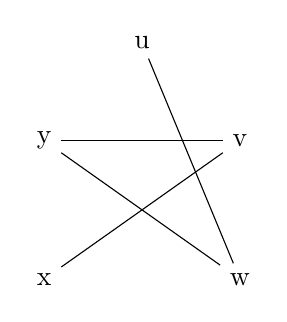
\begin{tikzpicture}[node distance=5em]
		\node (u) at (0,0) {u};
		\node (y) [below left of=u] {y};
		\node (v) [below right of=u] {v};
		\node (x) [below of=y] {x};
		\node (w) [below of=v] {w};

		\path[-] (y) edge(v);
		\path[-] (y) edge(w);
		\path[-] (u) edge(w);
		\path[-] (v) edge(x);
	\end{tikzpicture}
\end{equation}

We can see that this is correct because the union $E(G)\cup E(\bar{G})$ would lead to a complete graph.
In a complete graph, every vertex would have $(n-1)$ edges for $n$ nodes. 
Thus in the graph above each vertex would have $4$ edges.
By the corollary from the Degree Sum Formula, since each edge gets counted twice, we know that 
the complete graph would have $(4\times 5)/2 = 10$ edges.
If $G$ has six edges, then $\bar{G}$ will have four edges, none of which is present in $G$.
Then we can know that the graph above is the correct complement of $G$.

\section{Describe the definition of self-complementary.}
A graph is self-complementary when it is isomorphic to its complement.
An isomorphism on two graphs $G$ and $H$ means that we can map the $V(G)$ to $V(H)$ and $E(G)$ to $E(H)$ such that
each edge  in $E(G)$ is mapped to an equivalent edge in $E(H)$.
Essentially, an isomorphism means two graphs have the same structure, and a self-complementary graph would be identical
in structure to its own complement.

\section{What is a walk? What is a trail? Is a walk a trail?}
A \textbf{walk} is an ordered list of edges and vertices $v_0, e_1, v_1, \dots,v_{i-1}, e_{i}, v_{i}$ such that edge $e_i$
connects vertices $v_{i-1}, v_i$.
We can think of a walk as ``traveling'' along an edge from one vertex to another.
A \textbf{trail} is a walk with no repeated edges.
All trails are walks, since they are just a sequence of edges and vertices, but not all walks are trails, as some
can have repeated edges.

\section{Describe the degree-sum formula.}
The degree-sum formula in Eq.~\ref{eq:DSF} relates the sum of the degrees of $G$ to the number of edges.
It states that the total sum of the degrees is exactly twice the number of edges, because when counting all the degrees,
the edge between $u,v$ is counted exactly twice, once for each vertex.
There are interesting results that come from this equation as corollaries, such as the number of vertices with odd
degrees has to be even.
We used this result to show the non-existence of a specific graph.

Some other interesting results are the average number of vertices of a graph, which lies between $\delta(G)$ and $\Delta(G)$,
and the number of edges in a $k$-regular graph.

\section{Prove or disprove: If $u$ and $v$ are the only vertices of odd degree in a graph $G$, then $G$ contains a $u-v$ path.}
A \textbf{path} is a sequence of edges which connects two vertices, with all vertices being distinct.
According to Theorem 1.2.33 in the textbook, for a connected nontrivial graph with $2k$ odd vertices, there are at least
$\max\{k, 1\}$ trails that decompose the graph.
In this example, $k=1$ since it is given there are $2$ vertices with odd degrees.
A trail will contribute $2$ to all the non-endpoint vertices, and $1$ otherwise.

Since there is at least a trail that decomposes $G$, we can convert this trail into a path.
Trails do not have repeated edges, but \emph{can} have repeated vertices.
If vertex $v_i$ in the trail is repeated, we can remove the k-length cycle $v_i,\dots,v_{i+k}$, and end up with a path.

\section{(True or False) Every disconnected graph has an isolated vertex.}
This statement is \textbf{false}.
A graph is \textbf{connected} when there is a path between any two vertices $u,v$, and \textbf{disconnected} when there is
at least one pair of vertices without a path.
I graph with an isolated vertex would be disconnected, since an isolated vertex has degree $0$ and so no path exists
between this vertex and any other.
However, any graph with more than one component also is disconnected and may not have an isolated vertex.

For example, the following graph is disconnected with two components,
yet no isolated vertex.

\begin{equation}
		\begin{tikzpicture}[node distance=5em]
			\node (u) at (0,0) {u};
			\node (y) [below of=u] {y};
			\node (w) [right of=u] {w};
			\node (x) [below of=w] {x};

			\path[-] (u) edge (y);
			\path[-] (w) edge (x);
		\end{tikzpicture}
\end{equation}

\section{Prove or disprove. If every vertex of a simple graph $G$ has degree 2, then $G$ is a cycle.}
Lemma 1.2.5 in the textbook states that if every vertex in $G$ has degree at least 2, then $G$ contains
a cycle.
Thus we know that the graph contains a cycle, and we want to show the graph \emph{is} a cycle.
If every node has degree $2$, then we can think of a path that travels along $G$ from vertex $v_i$ to 
$v_{i+1}$.
A path contributes $2$ to a node's degree, so all the non-endpoint vertices in the path will 
have degree 2, except for the endpoints of the path which both have degree $1$.
To make every vertex have degree $2$, we would need an edge connecting $v_1,v_n$, which would create
a cycle for the entire graph.
Thus, if every node has degree $2$, then the graph has to be a cycle.
\end{document}
